\section{Начало работы в Python 3 и Wing IDE 101}

\subsection{О версиях Python}

Сейчас существуют две основных ветки (версии) развития языка Python (питон): Python 2 и Python 3. 
Версия~2 считается устаревающей, версия~3 "--- более новой и современной. 
Мы будем изучать именно версию~3. Версия~2 существенно отличается от версии 3, мы не будем обсуждать эти отличия.

В пределах как версии 2, так и версии 3 есть «подверсии», например, последняя версия из третьей ветки 
сейчас "--- версия 3.5.2 (не считая тех версий, которые находятся еще в разработке). 
В принципе, можно использовать более-менее любую версию питона из
третьей ветки, лучше как минимум 3.3, но если нет особенных причин, то устанавливайте последнюю
доступную вам версию.

\subsection{Установка Python}
Python — это свободное кросс-платформенное программное обеспечение, поэтому его можно легко
скачать с официального сайта, можно свободно распространять, и можно установить на все современные операционные
системы.

Чтобы установить Python под Windows, скачайте программу установки со странички курса или с официального сайта
(\verb`http://python.org`, через пункт Downloads; убедитесь, что вы скачиваете питон третьей версии для Windows). 
Установите Python с помощью этой программы, ничего сложного в установщике нет. 
Полезно установить питон куда-нибудь в корень диска, типа в \verb`C:\Python3`, а не в тот путь, 
который предлагается установщиком по умолчанию. Для этого при установке надо выбрать пункт типа Customize install 
и на одном из следующих экранов указать конкретный путь.

Если вы работаете в другой операционной системе, то разберитесь, как установить питон, самостоятельно. В Linux,
например, питон есть в репозиториях всех ведущих дистрибутивов, пакет обычно называется \verb`python3` 
(а просто \verb`python` "--- это питон второй версии).

\subsection{Установка Wing IDE}
Wing IDE "--- это, к сожалению, не свободное ПО, но у него существует официально бесплатная версия для 
образовательных целей, называется Wing IDE 101. Она доступна как для Windows, так и для Linux и OS X.

Все программы для установки можно скачать с официального сайта Wing IDE (\verb`http://wingware.com/`, 
через пункт Download --- Wing IDE 101); установщик под Windows также можно скачать со странички курса.
Установите Wing IDE с помощью этого установщика, ничего сложного в нем нет.

Wing IDE "--- это просто \textit{среда разработки} (IDE) для Python, т.е. удобный редактор программ,
позволяющий легко запускать программы с помощью питона (именно поэтому надо отдельно устанавливать сам 
Python "--- Wing IDE его не включает в себя). В принципе, вы можете использовать и какую-нибудь другую 
среду разработки, но тогда разбирайтесь с ней сами. В частности, сам Python включает простенькую среду 
разработки Python IDLE, ее описание вы можете встретить во многих  книжках по Python,
но она слишком простая и потому не очень удобная.

\subsection{Проверка установки}
Запустите Wing IDE. Появится окошко, похожее на показанное на рис. \ref{wing-0}а. 

Во-первых, убедитесь, что в правом нижнем углу, на панели, озаглавленной Python Shell, 
появился текст, похожий на приведенный на рисунке; в частности, там должна быть
указана версия питона, которую вы устанавливали. Убедитесь, что это версия 3 (на рисунке это версия 3.5.2).
Если это не так, то попробуйте через меню Edit --- Configure Python указать путь к питону вручную
(см. рис. \ref{wing-0}б) "--- в пункте Python Executable надо указать что-нибудь типа \verb`C:\Python3\python.exe`,
если вы установили питон в каталог \verb`C:\Python3`, возможно, также в список Python Path надо добавить 
\verb`C:\Python3`. Возможно, вам придется поэкспериментировать, чтобы найти правильные настройки. 
Если у вас на компьютере установлены обе версии питона (и 2, и 3), то, возможно, Wing IDE по умолчанию
«подцепит» версию 2, тогда тоже вручную укажите, что вам надо работать с версией 3.

Если у вас не получается, напишите мне, указав, куда вы установили питон, и прислав скриншоты основного окна
Wing IDE и диалога Edit — Configure Python.

\subsection{Первая программа}
В основном меню Wing IDE выберите пункт File --- New. Появится окно для редактирования текста программы. В этом окне наберите следующий текст (рис. \ref{first-prg}):

\begin{verbatim}
print("Test", 2*2)
\end{verbatim}
(Здесь \verb`"` "--- это символ кавычек.)

Убедитесь, что опечаток нет. Сохраните программу: нажмите Ctrl-S или выберите пункт меню File --- Save As. 
Wing IDE предложит выбрать имя файла для сохранения, для первой программы можно выбрать любое имя.


\begin{figure}[p]
\centerline{
а) 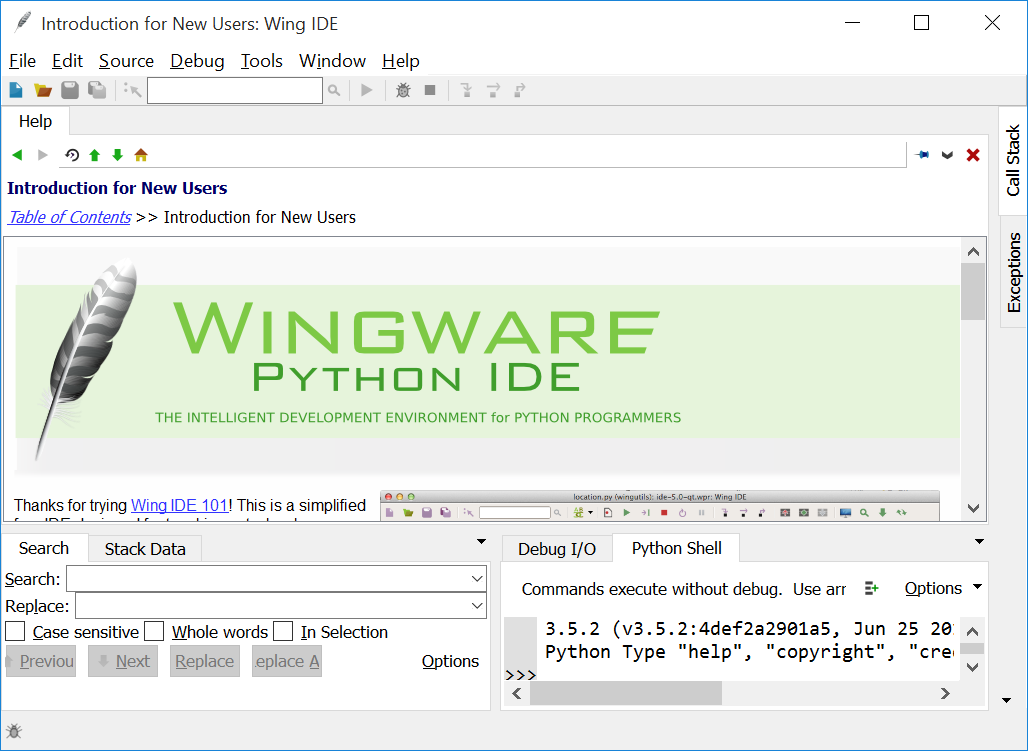
\includegraphics[width=8cm]{0_quick_start/wing_ide_0.png}\qquad 
б) 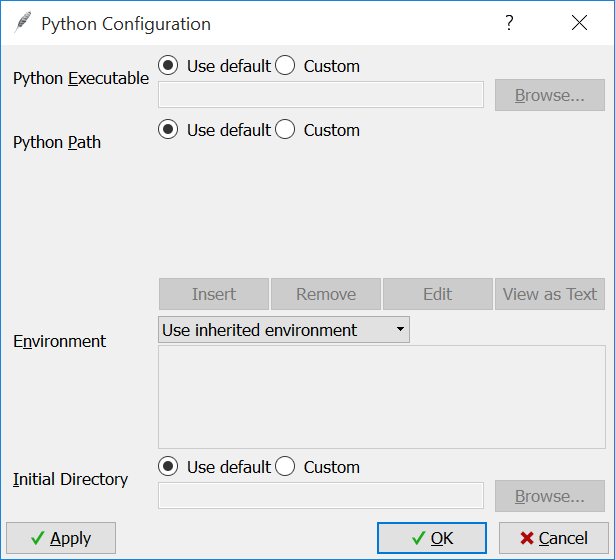
\includegraphics[width=6cm]{0_quick_start/wing_ide_config.png}
}
\caption{Основное окно Wing IDE}
\label{wing-0}
\end{figure}

\begin{figure}
\centerline{
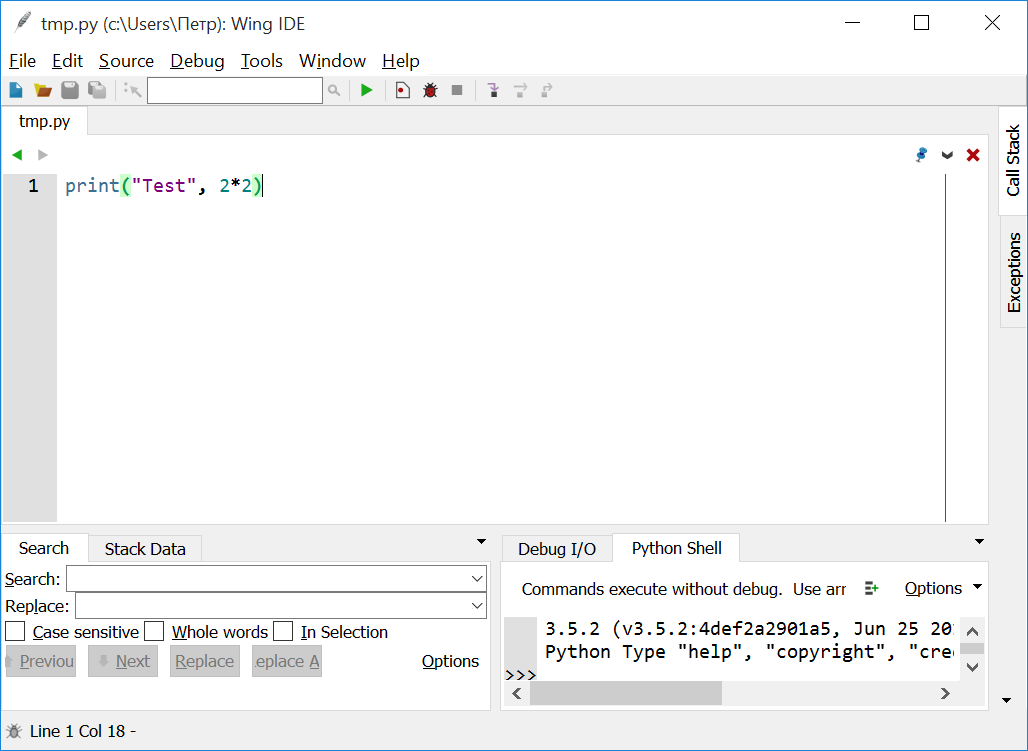
\includegraphics[width=8cm]{0_quick_start/wing_ide_1.png}
}
\caption{Простейшая программа}
\label{first-prg}
\end{figure}

После этого запустите программу, нажав на кнопку с зеленым треугольничком---стрелочкой на панели инструментов над 
текстом программы. Результат выполнения программы появляется в правой нижней части экрана, в панели «Python Shell»
А именно, там вы можете увидеть один из двух возможных результатов, показанных на рис. \ref{output}.
Если там появилась надпись «Test 4» (как на рис \ref{output}а), значит, все хорошо, программа успешно выполнилась. 
Если же там появился  (как на рис. \ref{output}б) длинный текст со словами «Traceback» (в начале) 
и «Error» (в конце), значит, в вашей программе есть ошибки.
Подробнее про ошибки ниже (раздел \ref{sec:ce}), а пока, если вы увидели ошибку,
то просто внимательно проверьте, не ошиблись ли вы где-нибудь в наборе программы. 

\begin{figure}
\centerline{
а) 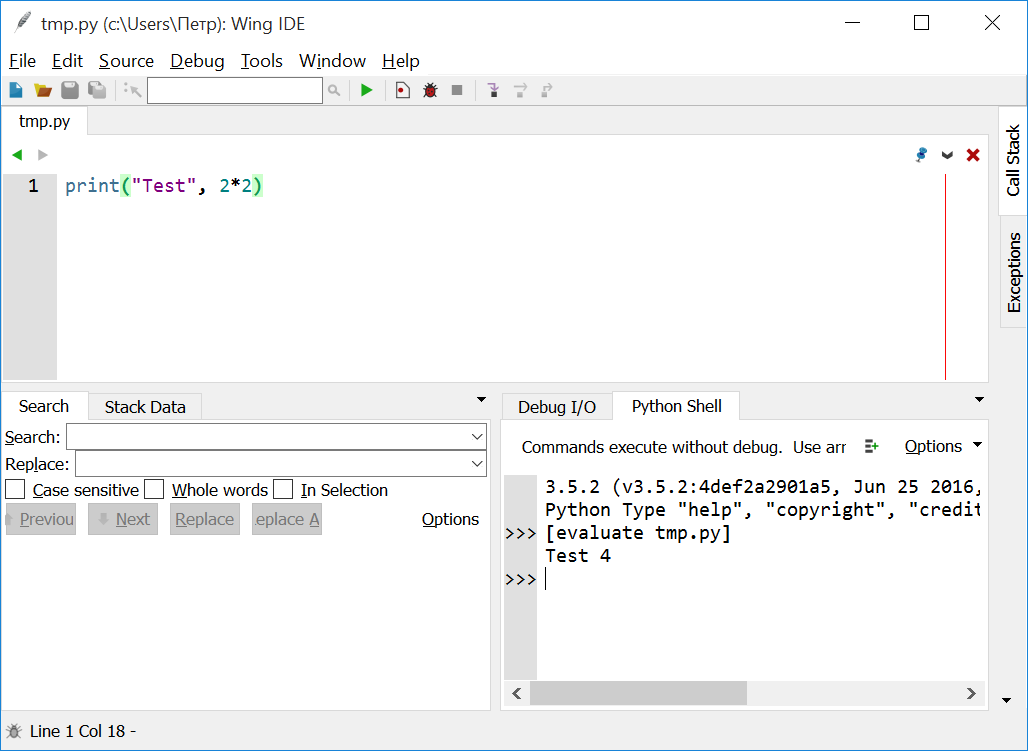
\includegraphics[width=8cm]{0_quick_start/wing_ide_2.png} \qquad
б) 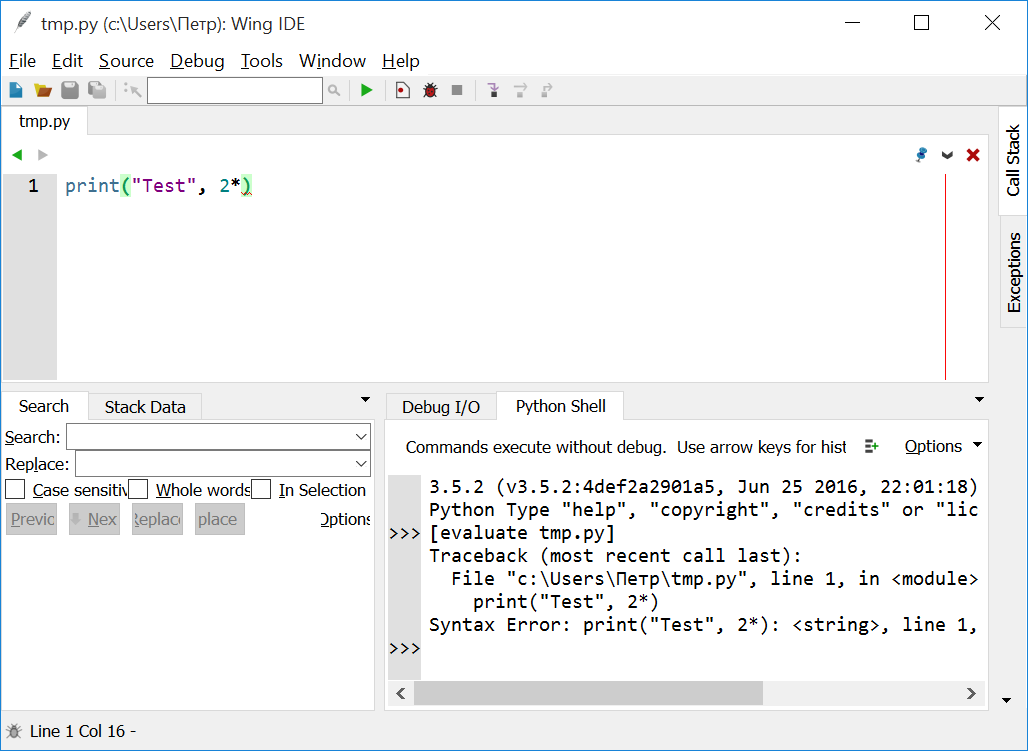
\includegraphics[width=8cm]{0_quick_start/wing_ide_3.png}
}
\caption{Вывод программы}
\label{output}
\end{figure}

Добейтесь того, чтобы ваша программа отработала успешно (внимательно проверив, не допустили ли вы ошибок), 
и посмотрите, что же именно пишется в этом окошке «Python Shell».
Там, во-первых, виден заголовок питона (включающий номер версии), дальше строка \verb`>>> [evaluate tmp.py]` 
(вместо \verb`tmp.py` здесь будет имя файла, куда вы сохранили программу). 
Эта строка была выведена в тот момент, когда Wing IDE начал запускать вашу программу. 
И, наконец, есть строка «\verb`Test 4`», которую и напечатала наша программа. 
Почему она напечатала именно это, обсудим чуть ниже.

Позапускайте программу (зеленой стрелочкой) ещё несколько раз и посмотрите на результаты. Вы увидите что, 
Wing IDE каждый раз печатает строку «\verb`evaluate...`» перед запуском программы, 
потом программа печатает свою строку.
Вывод программы перемешивается с выводом Wing IDE — ничего страшного, это нормально.

Можно также запускать программу нажатием на кнопку с картинкой типа красного жучка. 
Это немного другой режим запуска, более удобный для поиска ошибок. Попробуйте позапускать и так, и так, 
посмотрите на отличия (основное отличие пока "--- при запуске через «красного жучка» вывод предыдущих программ затирается).

\subsection{Ошибки в программе}
\label{sec:ce}
В вашей программе могут быть серьёзные ошибки — такие, что питон «не понимает», что вы от него хотите 
(а могут быть и не столь серьёзные — программа отработает как бы нормально, но выдаст неверный результат). 
В случае таких серьезных ошибок питон выдаст сообщение, похожее на показанное на рис. \ref{output}б.
Оно обычно начинается со слова Traceback, а ближе к концу в нем есть слово Error.

С ошибками удобнее разбираться, запуская программу в режиме «красного жучка». В таком случае Wing IDE 
подсвечивает строку около ошибки красным, а подробную информацию пишет в особом окошке справа.

Пока для вас важным будет то, какую строку Wing IDE подсветила красным "--- примерно в том месте и ошибка. Важен также
текст («сообщение об ошибке»), обычно содержащий слово «Error» (в нашем случае «\verb`Syntax Error ...`»),
там же рядом указан и номер строки с ошибкой («\verb`line 1`»).
Поначалу сообщения об ошибке сложно понимать, но со временем вы выучите наиболее часто встречающиеся 
и будете сразу понимать, что не так.

А пока посмотрите внимательно на строчку, которую питон подсветил красным (при запуске через «жучка»), 
и на строчки рядом "--- и попробуйте 
понять, что там не так. В примере на рисунке я забыл вторую цифру 2 (в результате чего питону стало непонятно,
на что надо умножать). (В примере на рисунке я запускал программу через зеленую стрелочку, а не через «красного
жучка», поэтому там нет подсвеченной красным строки.)

Имейте в виду, что питон не телепат и не может точно определить, где вы допустили ошибку. 
Он подсвечивает красным ту строку, где текст программы впервые разошёлся с правилами языка. 
Поэтому бывает, что на самом деле ваша ошибка чуть выше, чем подсвеченная строка (а иногда "--- и намного выше). 
Но тем не менее место, куда питон ставит курсор, обычно бывает полезно при поиске ошибки.

Попробуйте в своей программе поделать разные ошибки и посмотрите, как на них отреагирует питон. 

\subsection{Как работает эта программа}

Давайте разберём, как эта программа работает. Напомню её текст:
\begin{verbatim}
print("Test", 2*2)
\end{verbatim}

Вообще, любая программа "--- это, в первую очередь, последовательность команд, которые программист 
даёт компьютеру, а компьютер будет последовательно их выполнять. 

В нашей программе одна команда "--- \verb`print("Test", 2*2)`. Команда 
\verb`print` обозначает «вывести на экран» (английское слово `print' обозначает печатать). 
В скобках после слова \verb`print` указываются, как 
говорят, \textit{аргументы} команды. Они разделяются запятыми, в данном случае у команды два 
аргумента: первый "--- \verb`"Test"`, и второй "--- \verb`2*2`. 

Если аргументом команды \verb`print` является некоторая строка, заключённая в кавычки (символы \verb`"`), то 
команда \verb`print` выводит эту строку на экран как есть (без кавычек). Поэтому первым делом наша команда 
выводит на экран текст «\verb`Test`».

Вторым аргументом команды \verb`print` в нашем примере является арифметическое выражение 
\verb`2*2`. Если аргументом команды (любой команды, не обязательно именно \verb`print`, 
просто других мы 
пока не знаем) является арифметические выражение, то компьютер сначала вычислит его, а потом 
передаст команде. Поэтому в данном случае сначала компьютер вычислит $2\cdot 2$, получит 4, а потом 
передаст результат команде \verb`print`, которая выведет его на экран. 

Команда \verb`print` разделяет выводимые элементы пробелами, поэтому между \verb`Test` и \verb`4`
выведен пробел.

В итоге получается, что наша программа выводит \verb`Test 4`.

\subsection{Использование питона как калькулятора}

Таким образом можно использовать питон как калькулятор. Например, если надо посчитать значение 
выражения $7+3\cdot(8-2)$, то можно написать команду \verb`print(7+3*(8-2))`, 
после чего запустить программу "--- и на экран будет выведен результат. Обратите 
внимание, что скобки учтутся корректно и порядок действий будет правильный. Две скобки в конце команды "--- это одна 
является частью выражения, а вторая заканчивает список аргументов команды \verb`print`.

В выражениях можно использовать следующие операторы:
\begin{itemize}
\item \verb`+` и \verb`-` "--- сложение и вычитание (в том числе то, что называется \textit{унарный} минус для записи отрицательных чисел: чтобы написать $2\cdot(-4)$, надо написать \verb`2*(-4)`);
\item \verb`*` "--- умножение;
\item \verb`/` "--- деление («честное», например, $5/2=2.5$);
\item \verb`//` (это два символа \verb`/` подряд) и \verb`%` "--- это деление с остатком. 
Вспомните младшие классы и деление с остатком: 16 разделить на 3 будет 5 («неполное частное») и в остатке 1. 
Вот \verb`//` вычисляет неполное частное, а \verb`%` "--- остаток. Пишется так: \verb`16 // 3` и \verb`16 % 3`, 
как будто \verb`//` и \verb`%`{} "--- это символ операции, а-ля плюс или звёздочка. 
(Пробелы вокруг \verb`//` и \verb`%` не обязательны, но на питоне так принято.) При работе 
с отрицательными числами результат может показаться вам неожиданным, но это мы обсудим потом.
\item Скобки (только круглые) работают для группировки операций, можно использовать вложенные скобки, например, \verb`2*(3-(4+6))`.
\end{itemize}

Кроме того, есть так называемые \textit{функции}:
\begin{itemize}
\item Запись \verb`abs(-3)` обозначает взятие числа по модулю: $|{-}3|$. Обратите внимание: пишется сначала \textit{имя функции} (в данном случае \verb`abs`), а потом в скобках "--- от чего взять эту функцию (от чего взять модуль в данном случае). То, что в скобках, аналогично командам называется \textit{аргументом функции}.
\item Аналогично, запись \verb`sqrt(4)` обозначает взятие квадратного корня (если не знаете, что это такое, то пока пропустите этот пункт), но, поскольку эта операция бывает нужна несколько реже, то чтобы ее использовать, в начале программы надо написать магическую строку \verb`from math import *`. Программа получается, например, такая:
\begin{verbatim}
from math import *
print(sqrt(4))
\end{verbatim}
\end{itemize}

Все эти операции можно комбинировать. Например, команда \verb`print( (20 * 3) + sqrt( 2 + abs(5 - 7) ) )` выведет на экран значение выражения $20\cdot 3 + \sqrt{2+|5-7|}$. Пробелы в команде поставлены, чтобы проще было читать; вообще, в питоне пробелы можно ставить в любом разумном месте (внутри названий команд и чисел нельзя, но около скобок, знаков препинания и прочих символов можно), но рекомендуется ставить их как минимум вокруг знаков действий.

В одной программе можно вычислять несколько выражений. Например, программа
\begin{verbatim}
print(2 * 2, 2 + 2)
print(3 * 3)
\end{verbatim}
вычисляет три выражения. Первая команда \verb`print` выводит на экран две четвёрки, разделённых 
пробелом. Вторая команда просто выводит одно число 9. Оно будет выведено на отдельной строке, т.к. каждая команда \verb`print` выводит одну строку.

\subsection{Простейший ввод и вывод. Переменные}

Но не очень интересно писать программы, которые всегда выводят одно и то же. Хочется, чтобы программа что-нибудь запрашивала у пользователя, и работала с учётом того, что пользователь ввёл. Давайте, например, напишем программу, которая будет спрашивать у пользователя два числа и выводить на экран их сумму.

Но для этого нам придётся научиться ещё одной важной вещи. Когда пользователь вводит два числа, программе надо их как-то запомнить, чтобы потом сложить между собой и результат вывести на экран. Для этого у компьютера есть память (оперативная память). Программа может использовать эту память и положить туда числа, введённые пользователем. А потом посмотреть, что там лежит, сложить эти два числа, и вывести на экран.

Во многих языках, чтобы использовать память, надо особо попросить компьютер об этом. В питоне другой подход:
питон достаточно умен, чтобы самому догадаться, что вам нужна память. Давайте напишем следующую программу:

\begin{verbatim}
a = input()
print("(", a, ")")
\end{verbatim}

Прежде чем мы разберем, что обозначают все эти команды, наберите эту программу и попробуйте ее запустить.
Сначала запустите «зеленой стрелочкой». В окошке Python Shell появится надпись «\verb`[evaluate ...]`»,
после чего будет моргать курсор, а наверху этого окошка будет надпись «Waiting for keyboard input»,
что обозначает «Ожидаем ввод с клавиатуры». Введите что-нибудь в этом окошке и нажмите Enter.
Вы тут же увидите, что то, что вы ввели, вывелось еще одной строчкой на экран,
только окруженное скобками (и с дополнительными пробелами).
Именно это и делает программа: она выводит на экран то, что вы ей вводите,
окружая это скобками и дополнительными пробелами.

Если вы запустите программу «красным жучком», то все будет аналогично, только текст вам надо
будет вводить в пустом окошке «Debug I/O», которое появится на месте окошка «Python Shell».

Теперь разберем, как эта программа работает.

Команда \verb`input()` обозначает «подожди, пока пользователь введет что-нибудь с клавиатуры, и запомни то, 
что он ввел». Но просто так попросить «запомнить» довольно бессмысленно, нам ведь потом надо будет как-то
сказать компьютеру, чтобы он вспомнил то, что он запомнил. Поэтому мы пишем \verb`a = input()`. Это 
обозначает «запомни то, что ввел пользователь, в памяти, и дальше это место в памяти 
мы будем называть буквой \verb`a`».
Соответственно, команда \verb`print(a)` обозначает «посмотри, что лежит в памяти, называемой буквой \verb`a`, 
и выведи это на экран», а команда \verb`print("(", a, ")")` обозначает «выведи сначала открывающую скобку, 
потом то, что лежит в \verb`a`, потом закрывающую скобку, и раздели это все пробелами»

Вот такие «места в памяти» называются \textit{переменные}. Т.е. говорят: «переменная \verb`a`». Говорят:
в первой строке мы считали, что ввел пользователь с клавиатуры, и записали это в переменную \verb`a`,
а во второй строке мы прочитали, что записано в переменной \verb`a`, и вывели это на экран.

В программе можно заводить несколько переменных. Простейший вариант может выглядеть так:
\begin{verbatim}
a = input()
b = input()
print(b, a)
\end{verbatim}

Эта программа считывает две строки, которые вводит пользователь, и выводит их, причем сначала вторую,
а потом первую.

Но мы хотели написать программу, которая выводит сумму двух чисел. Простой подход тут не сработает:
\begin{verbatim}
a = input()
b = input()
print(a + b)
\end{verbatim}
сделает вовсе не то, что вы могли ожидать: питон пока считает, что в \verb`a` и \verb`b` могут лежать
какие угодно строки, и не понимает, что вы имели в виду числа.

Чтобы объяснить, что вы имеете в виду числа, надо написать так:
\begin{verbatim}
a = int(input())
b = int(input())
print(a + b)
\end{verbatim}

Мы используем новую команду (точнее, функцию) "--- \verb`int`. Она обозначает: возьми то, что получилось у команды \verb`input()`
(т.е. ту строку, которую вводит пользователь), и преврати это в число. Пока это не надо до конца осознавать,
просто запомните, что, чтобы считать одно число, надо написать \verb`... = int(input())`, где на место
многоточия надо подставить имя той переменной, куда надо записать результат.

Запустите эту программу. В окошке ввода наберите какое-нибудь число, нажмите Enter, наберите второе число
и еще раз нажмите Enter. Вы увидете, что программа вывела их сумму.

Если вы этой программе попытаетесь ввести два числа на одной строке (т.е. введете «2 пробел 3 Enter»),
то программа выдаст ошибку. Еще бы: вы пропросили строку «\verb`2 3`» превратить в число (в одно!) и записать
в переменную \verb`a`, но ведь это не есть верная запись одного числа.

Чтобы вводить числа через пробел, надо использовать другую конструкцию:
\begin{verbatim}
a, b = map(int, input().split())
\end{verbatim}

Это пока магия, ее придется запомнить наизусть. Потом вы поймете, что здесь что значит. Обратите внимание, что
после слова \verb`int` тут нет скобок, а вот после \verb`input` и \verb`split` есть.

Так можно вводить сколько угодно чисел; например, чтобы считать четыре числа, вводимые в одной строке, надо написать
\begin{verbatim}
a, b, c, d = map(int, input().split())
\end{verbatim}

Переменные не обязательно называть \verb`a` и \verb`b`, можно использовать более-менее любые строки из
английских букв (есть некоторые исключения, но пока это не так важно); например, можно было назвать
переменные \verb`first` и \verb`second`, и т.п. Конечно, переменных можно делать столько, сколько вам понадобится;
вообще, переменные "--- это основная вещь, с которой работают программы.

Ещё несколько замечаний по нашей программе. Во-первых, программа не вывела на экран никаких 
«приглашений» типа «Введите a и b». Питон ничего за вас делать не 
будет; если вы хотите, чтобы программа вывела это на экран, то так и сделайте: 
\verb`print("Введите a и b")`. Но мы не будем выводить 
такие приглашения в наших программах, мы будем считать, что пользователь сам знает, что от него 
требуется. В задачах, которые вы будете решать, будет чётко написано, что надо вывести на экран 
"--- и ничего лишнего выводиться не должно. 

\subsection{Присваивания}

Пока мы умеем записывать в переменные только то, что пользователь ввел с клавиатуры.
На самом деле, намного чаще приходится записывать в переменные значения, которые
программа сама вычисляет. Для этого есть специальная команда, которая называется
\textit{присваивание} (и на самом деле мы ее уже видели):
\begin{verbatim}
a = 10
\end{verbatim}
обозначает «в переменную \verb`a` записать 10». 

Справа от знака «равно» можно писать любые выражения (например, \verb`a = 10 + abs(5 - 9)`). 
Более того, там же можно использовать другие переменные, в которые уже что-то записано.
Например, программа
\begin{verbatim}
a = 20
b = a + 10
print(b)
\end{verbatim}
выведет на экран 30 (потому что сначала в \verb`a` записывается 20, потом компьютер смотрит,
что записано в \verb`a`, прибавляет 10, и результат записывает в \verb`b`, потом
смотрит, что записано в \verb`b`, и выводит на экран.

Если в переменной уже было что-то записано, то после присваивания старое значение затирается:
\begin{verbatim}
a = 20
a = 30
\end{verbatim}
в результате в \verb`a` лежит 30, а про 20 все забыли.

Особый интересный вариант "--- справа можно упоминать ту же переменную, которая стоит слева "--- 
тогда будет использоваться ее предыдущее значение:
\begin{verbatim}
a = 20
a = a + 10
\end{verbatim}
обозначает «в \verb`a` запиши 20. Потом посмотри, что записано в \verb`a`, прибавь к этому 10
и то, что получится, запиши обратно в \verb`a`». В итоге в \verb`a` будет записано 30.

Та команда \verb`a = input()`, которую мы раньше видели, на самом деле тоже является присваиванием:
она говорит: «прочитай то, что пользователь ввел с клавиатуры, и запиши это в \verb`a`».

Слева от знака «равно» можно указывать несколько переменных через запятую. Тогда справа
тоже должно быть несколько значений через запятую (или специальные функции типа уже упоминавшейся \verb`map`,
но их мы подробнее пока обсуждать не будем):
\begin{verbatim}
a, b = 10, 20
\end{verbatim}
обозначает «в \verb`a` записать 10, а в \verb`b` — 20».

Запись «\verb`a = 10`» читается «\verb`a` присвоить 10». Не надо говорить «\verb`a` равно 10», 
т.к. «равно» — это не глагол, и не понятно, какое действие совершается. Более того,
если запись «\verb`a = a + 1`» прочитать с «равно», то получается «\verb`a` равно \verb`a` плюс один»,
что никак не похоже на команду, а скорее на уравнение, которое не имеет решений. Поэтому говорите
«присвоить», а не «равно».

Есть еще ряд полезных команд, которые совмещают арифметическое действие и присваивание. Например,
запись \verb`a += 10` обозначает \verb`a = a + 10` («увеличить \verb`a` на 10»). Аналогично можно
поступать с остальными арифметическими действиями: \verb`a /= 5` обозначает \verb`a = a / 5`,
\verb`a %= 5` обозначает \verb`a = a % 5`, и т.п.

\subsection{Язык программирования как конструктор}
Выше я рассказал ряд самых основных конструкций языка питон. Теперь ваша задача будет из этих конструкций,
как из конструктора, собирать программы. Относитесь к этому именно как к конструктору: 
все программирование "--- это сборка больших программ из таких отдельных команд.

\subsection{Что дальше?}

Во-первых, если вы еще этого не сделали, прочитайте на страничке курса все тексты в «шапке» курса, 
особенно раздел «Работа с сайтом...», после чего начинайте решать «Задачи на арифметические операторы». И двигайтесь дальше по разделу «Для начинающих».

И по любым вопросам пишите мне.
